


\section{Scrum}

Scrum is by defenition a framework within which people can address complex adaptive problems, while productively and creatively delivering products of the highest possible value\cite{scrumguides}. 


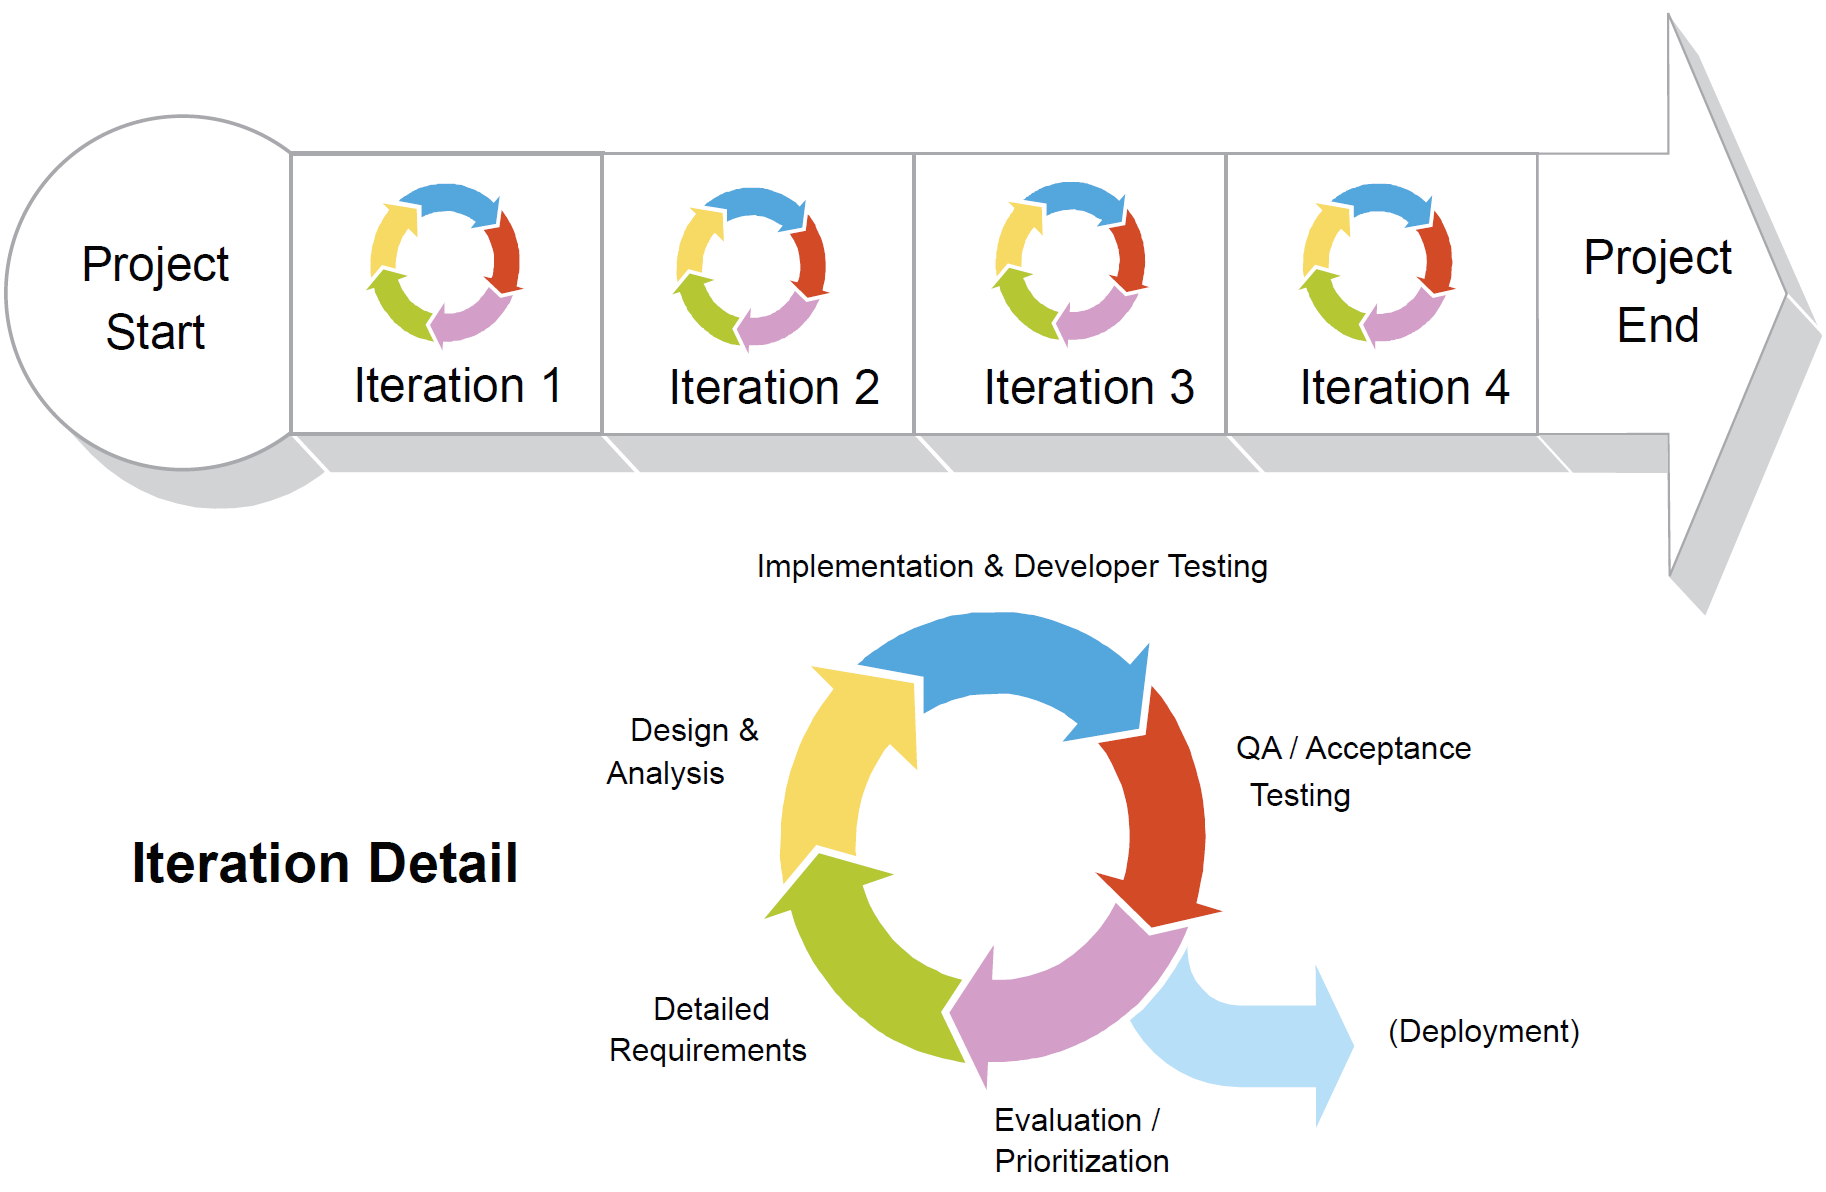
\includegraphics[scale=0.81]{VAPIQ-PICTURES/ScrumProcess.PNG}



Scrum is development model that coincides with the agile methodology. It provides a management framework for incremental product development using one or more cross-functional, self-organizing teams of about seven people each.\\

Agile is a movment that started 

It provides a structure of roles, meetings, rules, and artifacts. The roles involved is product owner, scrum master and team members. Each role represents a set of specific responsibilities and tasks.\\

Teams are
responsible for creating and adapting their processes within this
framework. 

Scrum uses fixed-length iterations, called Sprints, which are typically
two weeks or 30 days long. Scrum teams attempt to build a potentially
shippable (properly tested) product increment every
iteration\cite{ScrumReferenceCard}.
\\\\


\\\\
Scrum is easy to understand, but hard to implement.


\begin{comment}

%12 principles of agile
We follow these principles:
Our highest priority is to satisfy the customer
through early and continuous delivery
of valuable software.

Welcome changing requirements, even late in 
development. Agile processes harness change for 
the customer's competitive advantage.

Deliver working software frequently, from a 
couple of weeks to a couple of months, with a 
preference to the shorter timescale.

Business people and developers must work 
together daily throughout the project.

Build projects around motivated individuals. 
Give them the environment and support they need, 
and trust them to get the job done.

The most efficient and effective method of 
conveying information to and within a development 
team is face-to-face conversation.

Working software is the primary measure of progress.

Agile processes promote sustainable development. 
The sponsors, developers, and users should be able 
to maintain a constant pace indefinitely.

Continuous attention to technical excellence 
and good design enhances agility.

Simplicity--the art of maximizing the amount 
of work not done--is essential.

The best architectures, requirements, and designs 
emerge from self-organizing teams.

At regular intervals, the team reflects on how 
to become more effective, then tunes and adjusts 
its behavior accordingly.

Values of agile:

1. Individuals and Interactions Over Processes and Tools
2. Working Software Over Comprehensive Documentation
3. Customer Collaboration Over Contract Negotiation
4. Responding to Change Over Following a Plan

\end{comment}
